% Template adapted from https://github.com/jgm/pandoc-templates/blob/master/default.latex
% To be used with XeLaTex in memoiR
%%%%%%%%%%%%%%%%%%%%%%%%%%%%%%%%%%%%%%%%%%%%%%%%%%%%%%%%%%%%%%%%%%%%%%%%%%%%%%%%%%%%%%%%%

% Options for packages loaded elsewhere
\PassOptionsToPackage{unicode=true}{hyperref}
\PassOptionsToPackage{hyphens}{url}
\PassOptionsToPackage{dvipsnames,svgnames*,x11names*}{xcolor}
% Right to left support


\documentclass[
  12pt,
  american,
  a4paper,
  extrafontsizes,onecolumn,openright
  ]{memoir}

% Double (or whatever) spacing

% Math
\usepackage{amssymb, amsmath}
% mathspec: arbitrary math fonts
\usepackage{unicode-math}
\defaultfontfeatures{Scale=MatchLowercase}
\defaultfontfeatures[\rmfamily]{Ligatures=TeX,Scale=1}

% Fonts
\usepackage{lmodern}
\usepackage{fontspec}
% Main font
% Specific sanserif font
% Specific monotype font
% Specific math font
% Chinese, Japanese, Corean fonts

% Use upquote for straight quotes in verbatim environments
\usepackage{upquote}
% Use microtype
\usepackage[]{microtype}
\UseMicrotypeSet[protrusion]{basicmath} % disable protrusion for tt fonts

% Verbatim in note

% Color links
\usepackage{xcolor}

% Strikeout

% Necessary for code chunks

% Listings package

% Tables
\usepackage{longtable,booktabs,tabu}
% Fix footnotes in tables (requires footnote package)
\IfFileExists{footnote.sty}{\usepackage{footnote}\makesavenoteenv{longtable}}{}

% Graphics
\usepackage{graphicx,grffile}
\graphicspath{{images/}}
\makeatletter
\def\maxwidth{\ifdim\Gin@nat@width>\linewidth\linewidth\else\Gin@nat@width\fi}
\def\maxheight{\ifdim\Gin@nat@height>\textheight\textheight\else\Gin@nat@height\fi}
\makeatother
% Scale images if necessary, so that they will not overflow the page
% margins by default, and it is still possible to overwrite the defaults
% using explicit options in \includegraphics[width, height, ...]{}
\setkeys{Gin}{width=\maxwidth,height=\maxheight,keepaspectratio}

% Prevent overfull lines
\setlength{\emergencystretch}{3em}  
\providecommand{\tightlist}{%
  \setlength{\itemsep}{0pt}\setlength{\parskip}{0pt}}

% Number sections for memoir (secnumdepth counter is ignored)
\setsecnumdepth{section}

% Set default figure placement to htbp
\makeatletter
\def\fps@figure{htbp}
\makeatother

% Spacing in lists
\usepackage{enumitem}

% Polyglossia
\usepackage{polyglossia}
\setmainlanguage{en-US}
\setotherlanguage{fr-FR}
\setotherlanguage{it}

% BibLaTeX
\usepackage[backend=biber,style=authoryear-ibid,isbn=false,backref=true,giveninits=true,uniquename=init,maxcitenames=2,maxbibnames=150,sorting=nyt,sortcites=false]{biblatex}
\addbibresource{references.bib}

% cslreferences environment required by pandoc > 2.7



%%%%%%%%%%%%%%%%%%%%%%%%%%%%%%%%%%%%%%%%%%%%%%%%%%%%%%%%%%
% memoiR format

% Chapter Summary environment 
\usepackage[tikz]{bclogo}
\newenvironment{Summary}
  {\begin{bclogo}[logo=\bctrombone, noborder=true, couleur=lightgray!50]{In a Nutshell}\parindent0pt}
  {\end{bclogo}}
% Syntax:
%
%```{block, type='Summary'}
% Deliver message here.
% ```

% scriptsize code 
\let\oldverbatim\verbatim
\def\verbatim{\oldverbatim\scriptsize}
% Applies to code blocks and R code results
% code chunk options size='scriptsize' applies only to R code and results
% if the code chunk sets a different size, \def\verbatim{...} is prioritary for code results 


% Layout
%%%%%%%%%%%%%%%%%%%%%%%%%%%%%%%%%%%%%%%%%%%%%%%%%%%%%%%%%%

% Based on memoir, style companion
\newcommand{\MemoirChapStyle}{daleif1}
\newcommand{\MemoirPageStyle}{Ruled}

% Space between paragraphs
\usepackage{parskip}
  \abnormalparskip{3pt}

% Adjust margin paragraphs vertical position
\usepackage{marginfix}


% Margins
%%%%%%%%%%%%%%%%%%%%%%%%%%%%%%%%%%%%%%%

% allow use of '-',+','/' ans '*' to make simple length computation
\usepackage{calc}

% Full-width figures utilities
\newlength\widthw % full width
\newlength{\rf}
\newcommand*{\definesHSpace}{
  \strictpagecheck % slower but efficient detection of odd/even pages
  \checkoddpage
  \ifoddpage
  \setlength{\rf}{0mm}
  \else
  \setlength{\rf}{\marginparsep+\marginparwidth}
  \fi
}

\makeatletter
% 1" margins for the front matter.
\newcommand*{\SmallMargins}{
  \setlrmarginsandblock{1.5in}{1.5in}{*}
  \setmarginnotes{0.1in}{0.1in}{0.1in}
 \setulmarginsandblock{1.5in}{1in}{*}
  \checkandfixthelayout
  \ch@ngetext
  \clearpage
  \setlength{\widthw}{\textwidth+\marginparsep+\marginparwidth}
  \footnotesatfoot
  \chapterstyle{\MemoirChapStyle}  % Chapter and page styles must be recalled
  \pagestyle{\MemoirPageStyle}
}

% 3" outer margin for the main matter
\newcommand{\LargeMargins}{\SmallMargins}
\makeatother

% Figure captions and footnotes in outer margins


% Main title page with filigrane
%%%%%%%%%%%%%%%%%%%%%%%%%%%%%%%%%%%%%%%%%%%%%%%%%%%%%%%%%%

% Text blocks
\usepackage[absolute,overlay]{textpos}
  \setlength{\TPHorizModule}{1mm}
  \setlength{\TPVertModule}{1mm}

\newcommand{\MainTitlePage}[2]{
  \SmallMargins % Margins
  \pagestyle{empty} % No header/footer
  \textblockorigin{\stockwidth-\paperwidth-\trimedge}{\trimtop} % recto
  \begin{textblock*}{2mm}(\spinemargin/2,\uppermargin/2)
    \rule{1pt}{\paperheight-\uppermargin}
  \end{textblock*}
  \begin{textblock*}{\paperwidth*2/3}(\paperwidth/5, \paperheight/5)
    \flushright
    \begin{Spacing}{3}
      {\fontfamily{qtm}\selectfont\fontsize{45}{45}\selectfont\textsc{\thetitle}}
    \end{Spacing}
  \end{textblock*}
    \begin{textblock*}{\paperwidth*2/3}(\paperwidth/5, \paperheight/2)
    \flushright
    {\fontfamily{qtm}\huge\theauthor}
  \end{textblock*}
    \begin{textblock*}{\paperwidth*2/3}[0, 1](\spinemargin, \uppermargin+\textheight)
    \normalfont\thedate
  \end{textblock*}
  ~\\ % Print a character or the page will not exist
  \newpage
  \textblockorigin{\trimedge}{\trimtop} % verso
  \begin{textblock*}{\textwidth}(\paperwidth-\spinemargin-\textwidth, \uppermargin)
    #1
  \end{textblock*}
  \begin{textblock*}{\textwidth}[0,1](\paperwidth-\spinemargin-\textwidth, \uppermargin+\textheight+\footskip)
    \centering
    
\includegraphics[width=\paperwidth/4]{logo}\\ \bigskip
    #2
  \end{textblock*}
  ~\\ % Print a character or the page will not exist
  \newpage
}

% Clear page and open an even one (\clearpage opens an odd one)
\newcommand{\evenpage}{
  \clearpage
  \strictpagecheck % slower but efficient detection of odd/even pages
  \checkoddpage
  \ifoddpage
    \thispagestyle{empty}
    ~\\ % Print a character or the page will not exist
    \newpage
  \else
    % do nothing
  \fi
}


%% PDF title page to insert
%%%%%%%%%%%%%%%%%%%%%%%%%%%%%%%%%%%%%%%%%%%%%%%%%%%%%%%%%%

\usepackage{pdfpages}


%% Bibliography
%%%%%%%%%%%%%%%%%%%%%%%%%%%%%%%%%%%%%%%%%%%%%%%%%%%%%%%%%%

\usepackage[strict,autostyle]{csquotes}
% Repeated citation as author-year-title instead of author-title (modification of footcite:note in verbose-inote.cbx)

%% Table of Contents
%%%%%%%%%%%%%%%%%%%%%%%%%%%%%%%%%%%%%%%%%%%%%%%%%%%%%%%%%%

% fix the typesetting of the part number
\renewcommand\partnumberlinebox[2]{#2\ ---\ }


% Fonts
%%%%%%%%%%%%%%%%%%%%%%%%%%%%%%%%%%%%%%%%%%%%%%%%%%%%%%%%%%


% Hyperref comes last
%%%%%%%%%%%%%%%%%%%%%%%%%%%%%%%%%%%%%%%%%%%%%%%%%%%%%%%%%%

\usepackage{hyperref}
\hypersetup{
  pdftitle={User's guide for Ecofog's Ecophysiology Lab},
  pdfauthor={Marion Boisseaux, Daniela Krebber, Tristan Lafont Rapnouil},
  colorlinks=true,
  linkcolor=Maroon,
  citecolor=Blue,
  urlcolor=Blue,
  breaklinks=true}

% Don't use monospace font for urls
\urlstyle{same}


% Title, author, date from YAML to LaTeX
%%%%%%%%%%%%%%%%%%%%%%%%%%%%%%%%%%%%%%%%%%%%%%%%%%%%%%%%%%

\title{User's guide for Ecofog's Ecophysiology Lab}

\author{Marion Boisseaux, Daniela Krebber, Tristan Lafont Rapnouil}

\date{2021-10-31}


% Include headers (preamble.tex) here
%%%%%%%%%%%%%%%%%%%%%%%%%%%%%%%%%%%%%%%%%%%%%%%%%%%%%%%%%%
% Add LaTeX code into the preamble of the document here
\hyphenation{bio-di-ver-si-ty sap-lings}


%%%%%%%%%%%%%%%%%%%%%%%%%%%%%%%%%%%%%%%%%%%%%%%%%%%%%%%%%%%%%%%%%%%%%%%%%
% memoiR dalef3 chapter style 
% https://ctan.crest.fr/tex-archive/info/latex-samples/MemoirChapStyles/MemoirChapStyles.pdf
\usepackage{soul}
\definecolor{nicered}{rgb}{.647,.129,.149}
\makeatletter
\newlength\dlf@normtxtw
\setlength\dlf@normtxtw{\textwidth}
\def\myhelvetfont{\def\sfdefault{mdput}}
\newsavebox{\feline@chapter}
\newcommand\feline@chapter@marker[1][4cm]{%
  \sbox\feline@chapter{%
    \resizebox{!}{#1}{\fboxsep=1pt%
	  \colorbox{nicered}{\color{white}\bfseries\sffamily\thechapter}%
	}}%
  \rotatebox{90}{%
    \resizebox{%
	  \heightof{\usebox{\feline@chapter}}+\depthof{\usebox{\feline@chapter}}}%
	{!}{\scshape\so\@chapapp}}\quad%
  \raisebox{\depthof{\usebox{\feline@chapter}}}{\usebox{\feline@chapter}}%
 }
\newcommand\feline@chm[1][4cm]{%
  \sbox\feline@chapter{\feline@chapter@marker[#1]}%
  \makebox[0pt][l]{% aka \rlap
    \makebox[1cm][r]{\usebox\feline@chapter}%
  }}
\makechapterstyle{daleif1}{
  \renewcommand\chapnamefont{\normalfont\Large\scshape\raggedleft\so}
  \renewcommand\chaptitlefont{\normalfont\huge\bfseries\scshape\color{nicered}}
  \renewcommand\chapternamenum{}
  \renewcommand\printchaptername{}
  \renewcommand\printchapternum{\null\hfill\feline@chm[2.5cm]\par}
  \renewcommand\afterchapternum{\par\vskip\midchapskip}
  \renewcommand\printchaptertitle[1]{\chaptitlefont\raggedleft ##1\par}
}
\makeatother


% End of preamble
%%%%%%%%%%%%%%%%%%%%%%%%%%%%%%%%%%%%%%%%%%%%%%%%%%%%%%%%%%


\begin{document}
\frontmatter

% Title page
%%%%%%%%%%%%%%%%%%%%%%%%%%%%%%%%%%%%%%%%%%%%%%%%%%%%%%%%%%

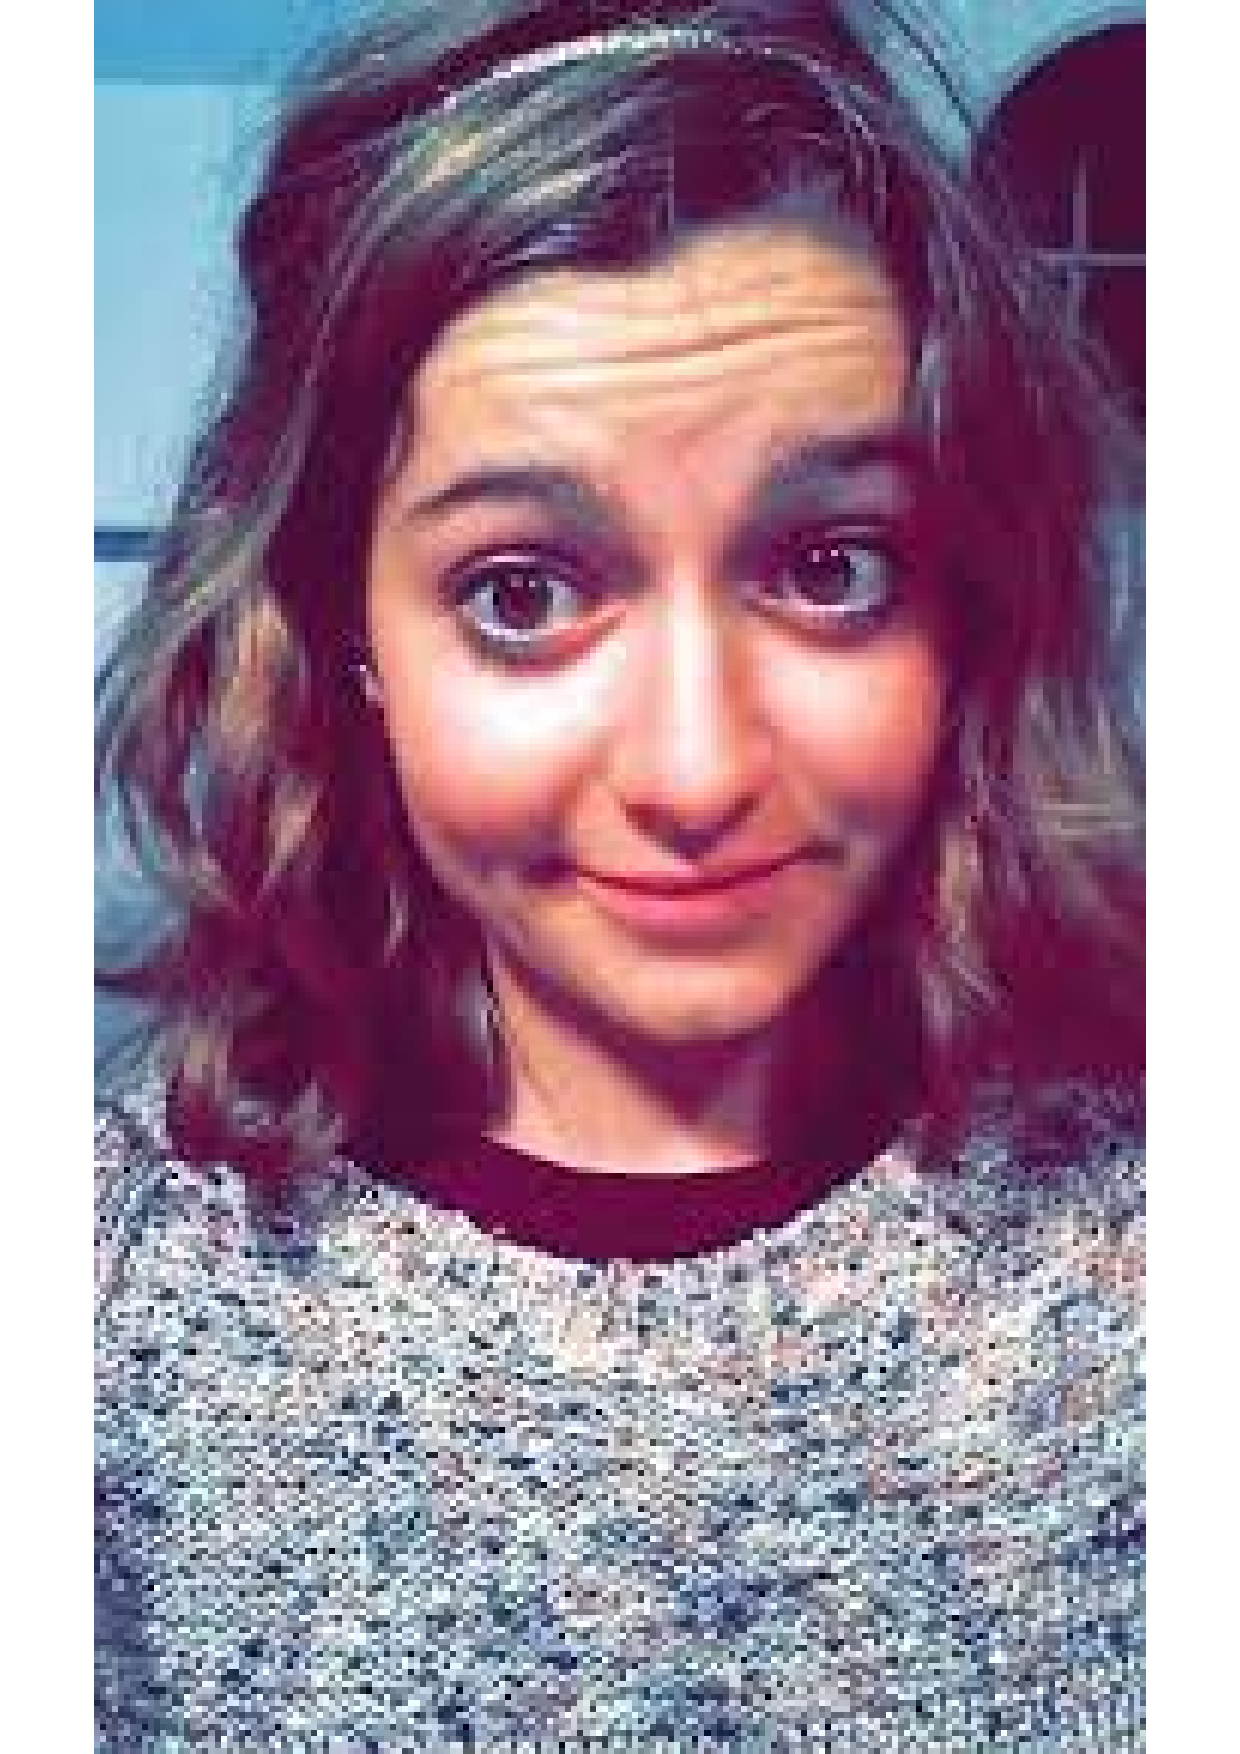
\includepdf[pages=1]{images/mariono.pdf}
\cleardoublepage

\MainTitlePage{This document is reproducible thanks to:

\begin{itemize}
  \item \LaTeX and its class memoir (\url{http://www.ctan.org/pkg/memoir}).
  \item R (\url{http://www.r-project.org/}) and RStudio (\url{http://www.rstudio.com/})
  \item bookdown (\url{http://bookdown.org/}) and memoiR (\url{https://ericmarcon.github.io/memoiR/})
\end{itemize}}{Name of the owner of the logo

\url{http://www.company.com}

An explanatory sentence.
Leave an empty line for line breaks.}


% Before Body
%%%%%%%%%%%%%%%%%%%%%%%%%%%%%%%%%%%%%%%%%%%%%%%%%%%%%%%%%%




% Contents
%%%%%%%%%%%%%%%%%%%%%%%%%%%%%%%%%%%%%%%%%%%%%%%%%%%%%%%%%%

\LargeMargins
{
\hypersetup{linkcolor=}
\setcounter{tocdepth}{2}
\tableofcontents
}


% Body
%%%%%%%%%%%%%%%%%%%%%%%%%%%%%%%%%%%%%%%%%%%%%%%%%%%%%%%%%%

\LargeMargins
\hypertarget{title-page}{%
\chapter{Title page\ldots{}}\label{title-page}}

Placeholder

\hypertarget{intro}{%
\chapter{Introduction}\label{intro}}

Plant functional traits are the features (morphological, physiological, phenological) that represent ecological strategies and determine \emph{describe?} how plants respond to environmental factors, affect other trophic levels and influence ecosystem properties. Variation in plant functional traits, and trait syndromes, has proven useful for tackling many important ecological questions at a range of scales, giving rise to a demand for standardized ways to measure ecologically meaningful plant traits. The importance of these topics dictates the urgent need for more and better data, and increases the value of standardized protocols for quantifying trait variation of different species, in particular for traits with power to predict plant- and ecosystem-level processes, and for traits that can be measured relatively easily (Pérez-Harguindeguy et al., 2013)

This handbook presents the different protocols used in the ecophysio lab. We therefore suggest the methodological principles for a more open and transparent science. This handbook not only includes updated methods for the trait measurements, but also includes the excel worksheets for data collection and the associated R-scripts to upload/clean the raw data.

\hypertarget{handbook-architecture}{%
\chapter{Handbook architecture}\label{handbook-architecture}}

This handbook is written for operational ends. As such, it is not a review or scientific paper thoroughly presenting each traits but rather a list of protocols associated with routinely measured traits in this lab.

Each chapter of this book correspond to one trait and associated measurement process.

\hypertarget{morpho-anatomy}{%
\section{Morpho-anatomy}\label{morpho-anatomy}}

\hypertarget{hydraulics}{%
\section{Hydraulics}\label{hydraulics}}

\hypertarget{fluorescence}{%
\section{Fluorescence}\label{fluorescence}}

\hypertarget{fluxes-and-gaz-exchange}{%
\section{Fluxes and gaz exchange}\label{fluxes-and-gaz-exchange}}

\hypertarget{microbial}{%
\section{Microbial}\label{microbial}}

\hypertarget{greenhouse-setups-and-tips}{%
\section{Greenhouse setups and tips}\label{greenhouse-setups-and-tips}}

\hypertarget{machine-info}{%
\section{Machine info}\label{machine-info}}

\hypertarget{root-morphology}{%
\section{Root Morphology}\label{root-morphology}}

\hypertarget{image-acquisition}{%
\subsection{Image Acquisition}\label{image-acquisition}}

\hypertarget{format}{%
\subsubsection{Format}\label{format}}

\hypertarget{scanner}{%
\subsubsection{Scanner}\label{scanner}}

\hypertarget{scan-process}{%
\subsubsection{Scan process}\label{scan-process}}

\hypertarget{flat-scan}{%
\paragraph{Flat scan}\label{flat-scan}}

\hypertarget{transparent}{%
\paragraph{Transparent}\label{transparent}}

\hypertarget{image-processing}{%
\subsection{Image processing}\label{image-processing}}

\hypertarget{winrhizo}{%
\subsection{WinRhizo}\label{winrhizo}}

\hypertarget{installation}{%
\subsubsection{Installation}\label{installation}}

\hypertarget{startup}{%
\subsubsection{Startup}\label{startup}}

\hypertarget{first-analysis}{%
\subsubsection{First analysis}\label{first-analysis}}

\hypertarget{calibration}{%
\subsubsection{Calibration}\label{calibration}}

\hypertarget{batch}{%
\subsubsection{Batch}\label{batch}}

\hypertarget{pixel-classification}{%
\subsubsection{Pixel classification}\label{pixel-classification}}

\hypertarget{output}{%
\subsubsection{Output}\label{output}}

\hypertarget{leaf-turgor-loss-point-pi_tlp}{%
\chapter{\texorpdfstring{Leaf turgor loss point, \(\pi_{tlp}\)}{Leaf turgor loss point, \textbackslash pi\_\{tlp\}}}\label{leaf-turgor-loss-point-pi_tlp}}

We assessed the leaf turgor loss point, \(\pi_{tlp}\) in MPa, from a previously established relationship with the osmotic potential at full hydration, \(\pi_{osm}\) in MPa. \(\pi_{osm}\) is linked to the equilibrium solute concentration value \(C_0\) (in mmol.kg\^{}\{-1\}) directly measured with a vapor pressure osmometer (Vapro 5600, Wescor, Logan, UT). This is referred as the \emph{osmometer method} (Bartlett et al.~2012a; Maréchaux et al.~2016).

\hypertarget{materials}{%
\section{Materials}\label{materials}}

\begin{itemize}
\tightlist
\item
  Vapor pressure osmometer (Vapro 5520, Wescor, Logan, UT)
\item
  Vapro software (Vapro Lab Report)
\item
  Fridge
\item
  Liquid Nitrogen
\item
  Ziplock bag\\
\item
  Paper towel
\item
  Distilled water
\item
  Metal tea ball
\item
  Tin foil
\item
  Needle\\
\item
  Liquid nitrogen gloves + goggles
\item
  Liquid nitrogen contenant
\item
  2 Tweezers
\item
  Cork borer
\end{itemize}

\hypertarget{methods}{%
\section{Methods}\label{methods}}

\hypertarget{installing-vapro-for-measurements}{%
\subsection{Installing Vapro for measurements}\label{installing-vapro-for-measurements}}

\begin{itemize}
\tightlist
\item
  Turn on Vapro the day before for the thermocouple's stability
\item
  Test Water Quality \emph{cf Vapro\_cheatsheet}
\item
  Clean
\item
  Calibration \emph{cf Vapro\_cheatsheet}
\item
  Control tests \emph{cf Vapro\_cheatsheet}
\item
  Verify temperature
\item
  Always have the black diamond at the center of the display
\end{itemize}

Used daily:
* clean beforehand
* select automatic mode (10 runs)

\hypertarget{sampling-on-the-field}{%
\subsection{Sampling on the field}\label{sampling-on-the-field}}

\begin{itemize}
\tightlist
\item
  Collect at least 3 healthy mature leaves on branch
\item
  Place them in sample ziplock bag with:

  \begin{itemize}
  \tightlist
  \item
    wet paper towel
  \item
    Exhale in bag to saturate in CO\textsubscript{2}
  \item
    Annotate bag with sample information
  \end{itemize}
\item
  Zip bag and stock in cooler
\end{itemize}

\hypertarget{lab-measurements}{%
\subsection{Lab measurements}\label{lab-measurements}}

\hypertarget{field-day}{%
\subsubsection{Field day}\label{field-day}}

\begin{itemize}
\tightlist
\item
  Recut branch under water
\item
  Replace in ziplock bag with wet paper towel
\item
  Put 24h in fridge to hydrate overnight
\end{itemize}

\hypertarget{n1-field-day}{%
\subsubsection{N+1 Field day}\label{n1-field-day}}

Vapro:

\begin{itemize}
\tightlist
\item
  check distilled water in vapro reservoir
\item
  clean
\item
  select automatic mode (10 runs)
\item
  make sure vapro software is on
\end{itemize}

Sample measurement:

\begin{itemize}
\tightlist
\item
  Sample from a leaf a 5 mm disc with a cork borer: \emph{avoid 1\textsuperscript{st} and 2\textsuperscript{nd} order veins to avoid apoplastic dilution that would lead to less negative osmometer values}
\item
  Wrap disc in tin foil
\item
  Immerse in liquid nitrogen for at least 2 min using metal tea ball
\item
  Puncture 10-15 times with needle
\item
  Place in vapro chamber
\end{itemize}

In total, disc are exposed to air for less than 40 seconds for all the steps.

\begin{itemize}
\item
  Record value C\textsubscript{0} when the difference between consecutive 2-min measurements fell below strictly 5 mmol.kg\textsuperscript{-1} after at least three runs.
\item
  If error! or Nr\_Run \textgreater{} 10 :
\item
  try a 2\textsuperscript{nd} cycle with same leaf
\item
  try a 3\textsuperscript{rd} cycle with another leaf
\item
  otherwise record \emph{NA}
\item
  Beware of the stuck leaf inside the vapro! If so \emph{cf Vapro\_cheatsheet}
\end{itemize}

\hypertarget{end-measurements}{%
\subsubsection{End measurements}\label{end-measurements}}

Clean Vapro

For more information on the vapro machine, please refer to the \emph{vapro cheatsheet} in the machine category.

\hypertarget{r-markdown}{%
\section{R Markdown}\label{r-markdown}}

\hypertarget{including-plots}{%
\section{Including Plots}\label{including-plots}}

\hypertarget{r-markdown-1}{%
\section{R Markdown}\label{r-markdown-1}}

\hypertarget{including-plots-1}{%
\section{Including Plots}\label{including-plots-1}}

\hypertarget{r-markdown-2}{%
\section{R Markdown}\label{r-markdown-2}}

\hypertarget{including-plots-2}{%
\section{Including Plots}\label{including-plots-2}}

\hypertarget{r-markdown-3}{%
\section{R Markdown}\label{r-markdown-3}}

\hypertarget{including-plots-3}{%
\section{Including Plots}\label{including-plots-3}}

\hypertarget{vapor-pressure-osmometer---vapro-5520-cheatsheet}{%
\chapter{Vapor pressure osmometer - Vapro 5520 cheatsheet}\label{vapor-pressure-osmometer---vapro-5520-cheatsheet}}

\begin{itemize}
\tightlist
\item
  \href{./document/machine/Vapro\%205520/Vapro_cheatsheet.pdf}{\textbf{\(\pi_{TLP}\)} vapro cheatsheet}
\end{itemize}

This template is based on \emph{Bookdown} and the \emph{Memoir} LaTeX class to allow writing a book, a report, a PhD thesis, etc. in \emph{R Markdown}.

The main file is \emph{index.Rmd} which contains the description of the book in its header. All other \emph{.Rmd} files in the folder contain a chapter.
The \emph{references.bib} file contains the bibliography.

This file will have to be deleted, as well as \emph{81-getting\_started.Rmd} and \emph{82-syntax.Rmd}: they have to be replaced by the content of the book.

To get started, create a new R project from this folder.
Then open \emph{index.Rmd} and click on the \emph{Build Book} button in the \emph{Build} window of Rstudio.


% Bibliography
%%%%%%%%%%%%%%%%%%%%%%%%%%%%%%%%%%%%%%%%%%%%%%%%%%%%%%%%%%

\backmatter
\SmallMargins

\printbibliography
\onecolumn


% Tables (of tables, of figures)
%%%%%%%%%%%%%%%%%%%%%%%%%%%%%%%%%%%%%%%%%%%%%%%%%%%%%%%%%%


\cleardoublepage
\LargeMargins
\listoffigures


% After-body (LaTeX code inclusion)
%%%%%%%%%%%%%%%%%%%%%%%%%%%%%%%%%%%%%%%%%%%%%%%%%%%%%%%%%%



% Back cover
%%%%%%%%%%%%%%%%%%%%%%%%%%%%%%%%%%%%%%%%%%%%%%%%%%%%%%%%%%%

% Even page, small margins, no running head, no page number.
\evenpage
\SmallMargins
\thispagestyle{empty}

\begin{normalsize}

\begin{description}

\selectlanguage{english}
\item[Abstract]
English abstract, on the last page.

This is the user's guide of EcoFoG's ecophysiology lab
\item[Keywords]
Keyword in English, As a list.
~\\

\end{description}

\end{normalsize}

\vspace*{\fill}
\centering
\includegraphics[width=.3\textwidth]{images/logo}

\end{document}
